\chapter{Текст программного кода Python-модуля нечеткого вывода с использованием технологии CUDA}\label{app:A}


%Для крупных листингов есть два способа. Первый красивый, но в нём могут быть
%проблемы с поддержкой кириллицы (у вас может встречаться в~комментариях
%и~печатаемых сообщениях), он представлен на листинге~\cref{lst:hwbeauty}.
%\begin{lstlisting}[
%	language=Python, % Syntax highlighting (optional)
%	caption={Модуль-обертка на языке Cython}, % Caption
%	label={lst:cython}
%]
\begingroup
\captiondelim{ } % разделитель идентификатора с номером от наименования
\begin{ListingEnv}
	\caption{Модуль-обертка на языке Cython}
	\label{lst:cython}
\end{ListingEnv}
\begin{minted}[fontsize=\footnotesize,tabsize=2,breaklines]{cython}
cdef extern from "tsfuzzy.hpp":
    cdef enum class ImplType:
        LUKASIEWICZ,
        REICHENBACH,
        YAGER,
        KLEENE_DIENES
    cdef enum class DefuzMethod:
        COG,
        COG_SIMPLE,
        MEOM
    void fuzzy_fit_impl(
        const float *points_means, const float *points_stds, const unsigned points_size, const unsigned point_dims,
        float *rules_means, float *rules_std, const unsigned rules_count,
        const ImplType impl_type, const DefuzMethod defuz_method,
        const unsigned ftv_discretization_size, const unsigned defuz_pso_population_size, const unsigned defuz_pso_iter_count,
        const unsigned rules_pso_population_size, const unsigned rules_pso_iterations_count
    )
    void fuzzy_predict_impl(
        const float *points_means, const float *points_stds, float *predictions, const unsigned points_size, const unsigned point_dims,
        const float *rules_means, const float *rules_std, const unsigned rules_count,
        const ImplType impl_type, const DefuzMethod defuz_method,
        const unsigned ftv_discretization_size, const unsigned defuz_pso_population_size, const unsigned defuz_pso_iter_count
    )

import numpy as np
cimport numpy as cnp
import pandas as pd

cnp.import_array()


cdef class TsFuzzy:
    cdef ImplType impl_type
    cdef DefuzMethod defuz_method
    cdef int ftv_discretization_size
    cdef int defuz_pso_population_size
    cdef int defuz_pso_iters_count
    cdef int rules_pso_population_size
    cdef int rules_pso_iterations_count
    cdef cnp.ndarray rules_means
    cdef cnp.ndarray rules_stds

    def __init__(
        self,
        rules_count: int, y_dims: int,
        impl_type: Literal["lukasiewicz", "reichenbach", "yager", "kleene_dienes"] = "lukasiewicz",
        defuz_method: Literal["cog", "cog_simple", "meom"] = "meom",
        ftv_discretization_size: int = 11, defuz_pso_population_size: int = 30, defuz_pso_iters_count: int = 100,
        rules_pso_population_size: int = 50, rules_pso_iterations_count: int = 150
    ):
        impl_type_map = {"lukasiewicz": ImplType.LUKASIEWICZ, "reichenbach": ImplType.REICHENBACH, "yager": ImplType.YAGER, "kleene_dienes": ImplType.KLEENE_DIENES}
        defuz_method_map = {"cog": DefuzMethod.COG, "cog_simple": DefuzMethod.COG_SIMPLE, "meom": DefuzMethod.MEOM}
        try:
            self.impl_type = impl_type_map[impl_type]
        except KeyError:
            raise ValueError("Invalid impl_type; expected 'lukasiewicz' or 'goguen'.")
        try:
            self.defuz_method = defuz_method_map[defuz_method]
        except KeyError:
            raise ValueError("Invalid defuz_method; expected 'cog', 'cog_simple', or 'meom'.")
        self.ftv_discretization_size = ftv_discretization_size
        self.defuz_pso_population_size = defuz_pso_population_size
        self.defuz_pso_iters_count = defuz_pso_iters_count
        self.rules_pso_population_size = rules_pso_population_size
        self.rules_pso_iterations_count = rules_pso_iterations_count
        self.rules_means = np.empty((rules_count, y_dims), dtype=np.float32)
        self.rules_stds = np.empty((rules_count, y_dims), dtype=np.float32)

    def fit(self, points_means_, points_stds_):
        assert points_means_.shape == points_stds_.shape
        cdef cnp.ndarray[cnp.float32_t, ndim=2, mode='c'] points_means = np.ascontiguousarray(points_means_, dtype=np.float32)
        cdef cnp.ndarray[cnp.float32_t, ndim=2, mode='c'] points_stds = np.ascontiguousarray(points_stds_, dtype=np.float32)
        cdef int points_size = points_means.shape[0]
        cdef int points_dims = points_means.shape[1]
        fuzzy_fit_impl(
            <const float*>points_means.data, <const float*>points_stds.data, points_size, points_dims,
            <float*>self.rules_means.data, <float*>self.rules_stds.data, self.rules_means.shape[0],
            self.impl_type, self.defuz_method, self.ftv_discretization_size, self.defuz_pso_population_size, self.defuz_pso_iters_count,
            self.rules_pso_population_size, self.rules_pso_iterations_count,
        )

    def predict(self, points_means_, points_stds_):
        assert points_means_.shape == points_stds_.shape
        cdef cnp.ndarray[cnp.float32_t, ndim=2, mode='c'] points_means = np.ascontiguousarray(points_means_, dtype=np.float32)
        cdef cnp.ndarray[cnp.float32_t, ndim=2, mode='c'] points_stds = np.ascontiguousarray(points_stds_, dtype=np.float32)
        cdef int points_size = points_means.shape[0]
        cdef int points_dims = points_means.shape[1]
        cdef cnp.ndarray[cnp.float32_t, ndim=1, mode='c'] predictions = np.empty(points_size, dtype=np.float32)
        fuzzy_predict_impl(
            <const float*>points_means.data, <const float*>points_stds.data, <float*>predictions.data, points_size, points_dims,
            <const float*>self.rules_means.data, <const float*>self.rules_stds.data, self.rules_means.shape[0],
            self.impl_type, self.defuz_method, self.ftv_discretization_size, self.defuz_pso_population_size, self.defuz_pso_iters_count,
        )
        return predictions

    def __getstate__(self):
        return {
            "impl_type": int(self.impl_type),
            "defuz_method": int(self.defuz_method),
            "ftv_discretization_size": self.ftv_discretization_size,
            "defuz_pso_population_size": self.defuz_pso_population_size,
            "defuz_pso_iters_count": self.defuz_pso_iters_count,
            "rules_means": np.asarray(self.rules_means),
            "rules_stds": np.asarray(self.rules_stds)
        }

    def __setstate__(self, state):
        from tsfuzzy import ImplType, DefuzMethod
        self.impl_type = ImplType(state["impl_type"])
        self.defuz_method = DefuzMethod(state["defuz_method"])
        self.ftv_discretization_size = state["ftv_discretization_size"]
        self.defuz_pso_population_size = state["defuz_pso_population_size"]
        self.defuz_pso_iters_count = state["defuz_pso_iters_count"]
        self.rules_means = np.ascontiguousarray(state["rules_means"], dtype=np.float32)
        self.rules_stds = np.ascontiguousarray(state["rules_stds"], dtype=np.float32)

    @staticmethod
    def fuzzify(
        y,
        wma = None, sample_std = 1.0
    ):
        # Compute the difference series d with length len(y)-1.
        d = pd.Series(y[1:] - y[:-1]) / np.sqrt(2)
        y = pd.Series(y)
        # Calculate deviations from d using ewm.
        computed_deviations = sample_std * d.ewm(alpha=0.7, adjust=False, min_periods=1).std()
        # Prepend the first computed deviation value so that deviations has the same length as y.
        deviations = pd.concat([pd.Series([computed_deviations.iloc[0]]), computed_deviations]).reset_index(drop=True)
        # Compute centers. Using min_periods=1 ensures that initial values are filled with the first computed mean.
        if wma is not None:
            centers = y.ewm(alpha=1 - wma, adjust=True, min_periods=1).mean()
        else:
            centers = y
        return centers, deviations
\end{minted}
\endgroup
Листинг реализации нечеткого вывода на языке CUDA C++ с использованием библиотек Kokkos и ArborX \cref{lst:hwplain}.
\begingroup
\captiondelim{ } % разделитель идентификатора с номером от наименования
\begin{ListingEnv}
\caption{Реализация нечеткого вывода на языке CUDA C++ с использованием библиотек Kokkos и ArborX}
\label{lst:cuda}
\end{ListingEnv}
\begin{minted}[fontsize=\footnotesize,tabsize=2,breaklines]{cuda}
template <typename RealT>
struct metrics
{
  std::size_t count = 0;
  RealT y_true_mean = 0;
  RealT y_true2_mean = 0;
  RealT mae = 0;
  RealT mape = 0;
  RealT mse = 0;
public:
  KOKKOS_INLINE_FUNCTION
  void operator()(RealT y_true, RealT y_pred)
  {
    y_true_mean = (y_true + count * y_true_mean) / (count+1);
    y_true2_mean = (y_true * y_true + count * y_true2_mean) / (count+1);
    mae = (Kokkos::abs(y_true - y_pred) + count * mae) / (count+1);
    mape = (Kokkos::abs(y_true - y_pred) / y_true + count * mape) / (count+1);
    mse = (Kokkos::pow(y_true - y_pred, 2) + count * mse) / (count+1);
    ++count;
  }

  KOKKOS_INLINE_FUNCTION
  RealT rmse() const { return Kokkos::sqrt(mse); }
  KOKKOS_INLINE_FUNCTION
  RealT ndei() const { return rmse() / std(); }
  KOKKOS_INLINE_FUNCTION
  RealT er2() const { return mse / var(); }

private:
  KOKKOS_INLINE_FUNCTION
  RealT var() const { return y_true2_mean - Kokkos::pow(y_true_mean, 2); }
  KOKKOS_INLINE_FUNCTION
  RealT std() const { return Kokkos::sqrt(var()); }
};


template <unsigned DIM, typename SomeMemoryTraits>
void fuzzy_infer(const Kokkos::View<ArborX::Point<DIM>*, Kokkos::OpenMP::array_layout, Kokkos::CudaSpace> &points_means_device,
                 const Kokkos::View<ArborX::Point<DIM>*, Kokkos::OpenMP::array_layout, Kokkos::CudaSpace> &points_stds_device,
                 Kokkos::View<float**, Kokkos::CudaSpace, SomeMemoryTraits> &predictions_population_device,
                 const Kokkos::View<ArborX::Point<DIM>**, Kokkos::CudaSpace, SomeMemoryTraits>& rules_means_population_device,
                 const Kokkos::View<ArborX::Point<DIM>**, Kokkos::CudaSpace, SomeMemoryTraits>& rules_stds_population_device,
                 const Kokkos::Random_XorShift64_Pool<Kokkos::Cuda> &warp_random_pool,
                 const Kokkos::Random_XorShift64_Pool<Kokkos::Cuda> &thread_random_pool,
                 const ImplType impl_type,
                 const DefuzMethod defuz_method,
                 const unsigned ftv_discretization_size,
                 const unsigned defuz_pso_population_size,
                 const unsigned defuz_pso_iterations_count,
                 const unsigned block_replication_count = 1) {

  const bool debug = (bool)get_env<int>("DEBUG", 0);
  const int DEBUG_FTV_RULE_IDX = get_env<int>("DEBUG_FTV_RULE_IDX", 0);
  const int DEBUG_V_STEP = get_env<int>("DEBUG_V_STEP", 50);
  const int DEBUG_SAMPLE_IDX = get_env<int>("DEBUG_SAMPLE_IDX", 10000);

  const unsigned rules_population_size = rules_means_population_device.extent(0);
  const unsigned rules_count = rules_means_population_device.extent(1);
  const unsigned warp_count = (44000 / (
    4 * (DIM*rules_count*2 + rules_count*ftv_discretization_size + rules_count*(DIM-1) + rules_count*3 + defuz_pso_population_size*5)
    + 1 * (rules_count*(DIM-1))
    + 1000
  ));
  assert(warp_count >= 1);

  // dprintf("rules_population_size = %u, block_replication_count = %u, warp_count = %u, rules_count = %u, ftv_discretization_size = %u, defuz_pso_population_size = %u\n", rules_population_size, block_replication_count, warp_count, rules_count, ftv_discretization_size, defuz_pso_population_size);
  Kokkos::TeamPolicy<Kokkos::Cuda> team_policy(rules_population_size * block_replication_count, 32 * warp_count);
  team_policy.set_scratch_size(0, Kokkos::PerTeam(44000));

  auto fuzzy_infer_block_lambda = [=] __device__ (const Kokkos::TeamPolicy<Kokkos::Cuda>::member_type &team) {
    // if (team.league_rank() == 0 && team.team_rank() == 0) {
    //   dprintf("gridDim = [%d %d %d] blockDim = [%d %d %d]\n",
    //     gridDim.x, gridDim.y, gridDim.z, blockDim.x, blockDim.y, blockDim.z);
    // }

    const int pso_idx = team.league_rank() / block_replication_count;
    const int warp_idx = team.team_rank() / 32;
    const int lane_idx = team.team_rank() % 32;
    auto warp_gen = warp_random_pool.get_state(team.league_rank() * warp_count + warp_idx);
    auto thread_gen = thread_random_pool.get_state(team.league_rank() * team.team_size() + team.team_rank());

    ScratchView<ArborX::Point<DIM>*> rules_means(team.team_shmem(), rules_count);
    ScratchView<ArborX::Point<DIM>*> rules_stds(team.team_shmem(), rules_count);
    // if (team.league_rank() == 0 && team.team_rank() == 0)
    //   printf("rules_count = %d, rules_means.extent(0) = %d, rules_stds.extent(0) = %d\n", (int)rules_count, (int)rules_means.extent(0), (int)rules_stds.extent(0));
    Kokkos::parallel_for(Kokkos::TeamThreadRange(team, rules_count), [=] __device__ (int j) {
      rules_means(j) = rules_means_population_device(pso_idx, j);
      rules_stds(j) = rules_stds_population_device(pso_idx, j);
    });
    __syncthreads();

    ScratchView<ArborX::Point<DIM>*> points_means(team.team_shmem(), warp_count), points_stds(team.team_shmem(), warp_count);

    // dprintf("league_rank: %d, team_rank: %d, pso_idx: %d, warp_idx: %d, lane_idx: %d, block_replication_count: %u, warp_count: %u\n",
    //     team.league_rank(), team.team_rank(), pso_idx, warp_idx, lane_idx, block_replication_count, warp_count);
    auto team_shmem_backup = team.team_shmem();
    for (int sample_idx = (team.league_rank() % block_replication_count) * warp_count + warp_idx;
        sample_idx < points_means_device.extent(0);
        sample_idx += block_replication_count * warp_count)
    {
      const_cast<ScratchSpace&>(team.team_shmem()) = team_shmem_backup;
      for (int i = lane_idx; i < DIM; i += 32) {
        points_means(warp_idx)[i] = points_means_device(sample_idx)[i];
        points_stds(warp_idx)[i] = points_stds_device(sample_idx)[i];
      }
      const auto point_means = Kokkos::subview(points_means, warp_idx);
      const auto point_stds = Kokkos::subview(points_stds, warp_idx);
      // if (lane_idx == 0) {
      //   printf("sample_idx = %d, warp_idx = %d, point = {[%f %f], [%f %f], [%f %f], [ %f %f], [%f %f]}\n",
      //   sample_idx,
      //   warp_idx,
      //   point_means()[0], point_stds()[0], 
      //   point_means()[1], point_stds()[1],
      //   point_means()[2], point_stds()[2], 
      //   point_means()[3], point_stds()[3],
      //   point_means()[4], point_stds()[4]
      //   // point_means()[5], point_stds()[5]
      //   );
      // }
      __syncwarp();

      using Kokkos::abs;
      using Kokkos::exp;
      using Kokkos::pow;
      using Kokkos::sqrt;
      using Kokkos::log;
      using Kokkos::round;
      
      ScratchView<float***> rules_reduced_ftv(team.team_shmem(), warp_count, rules_means.extent(0), ftv_discretization_size);
      // auto reduce_ftv_team_shmem_backup = team.team_shmem();

      {
        ScratchView<unsigned char***> rules_ftv_core_step(team.team_shmem(), warp_count, rules_means.extent(0), DIM-1);
        ScratchView<float***> rules_max_ftv(team.team_shmem(), warp_count, rules_means.extent(0), DIM-1);
        for (int rule_idx = lane_idx; rule_idx < rules_means.extent(0); rule_idx += 32) {
          auto reduced_ftv = Kokkos::subview(rules_reduced_ftv, warp_idx, rule_idx, Kokkos::ALL); // TODO // FIXME
          auto ftv_core_step = Kokkos::subview(rules_ftv_core_step, warp_idx, rule_idx, Kokkos::ALL);
          auto max_ftv = Kokkos::subview(rules_max_ftv, warp_idx, rule_idx, Kokkos::ALL);

          const auto &rule_means = rules_means(rule_idx);
          const auto &rule_stds = rules_stds(rule_idx);

          for (int dim = 0; dim < DIM-1; ++dim) {
            float a = rule_means[dim], b = rule_stds[dim];
            float c = point_means()[dim];
            ftv_core_step(dim) = min(max((int) round(exp(-pow((a-c)/b, 2)) * (ftv_discretization_size-1)), 0), ftv_discretization_size-1);
            // if (sample_idx == DEBUG_SAMPLE_IDX && rule_idx == DEBUG_FTV_RULE_IDX)
            //   dprintf("rule %d, dim = %d, [%f %f %f %f], ftv_core_step = %d\n", rule_idx, dim, a, b, c, point_stds()[dim], (int)ftv_core_step(dim));
            max_ftv(dim) = 0.f;
          }

          // Here task is to provide discretization shape most similar to the each of FTV shape cases
          for (int v_step = ftv_discretization_size; v_step > 0; ) {
            --v_step;
            float v = (float)v_step / (ftv_discretization_size-1);
            float v_max_ftv = 0.f, v_max_ftv_dim;
            bool is_growth_present = false;
            for (int dim = 0; dim < DIM-1; ++dim) {
              const float a = rule_means[dim], b = rule_stds[dim];
              const float c = point_means()[dim], d = point_stds()[dim];
              float ftv = (v_step == ftv_core_step(dim))
                ? 1.f
                : Kokkos::max(exp(-pow(((a - c) + b * sqrt(-log(v))) / d, 2)), exp(-pow(((a - c) - b * sqrt(-log(v))) / d, 2)));

              // if (rule_idx == DEBUG_FTV_RULE_IDX && v_step == DEBUG_V_STEP)
              //   printf("rule %d, v_step = %d, v = %f, dim = %d, ftv = %f\n", rule_idx, v_step, v, dim, ftv);
              if (ftv > max_ftv(dim)) {
                max_ftv(dim) = ftv;
                is_growth_present = true;
              }
              if (ftv > v_max_ftv) {
                v_max_ftv = ftv;
                v_max_ftv_dim = dim;
              }
            }
            float ftv_reduced = 1.f;
            for (int dim = 0; dim < DIM-1; ++dim) {
              if (!is_growth_present && (dim == v_max_ftv_dim)) {
                ftv_reduced = Kokkos::min(ftv_reduced, v_max_ftv);
              } else {
                ftv_reduced = Kokkos::min(ftv_reduced, max_ftv(dim));
              }
            }
            if (rule_idx == DEBUG_FTV_RULE_IDX && sample_idx == DEBUG_SAMPLE_IDX) {
              dprintf("rule %d, v_step = %d, v = %f, max_ftv = {%f %f %f %f %f}, v_max_ftv = %f, v_max_ftv_dim = %d, ftv_reduced = %f\n",
                rule_idx, v_step, v, max_ftv(0), max_ftv(1), max_ftv(2), max_ftv(3), max_ftv(4),
                v_max_ftv, (int)v_max_ftv_dim, ftv_reduced);
            }
            reduced_ftv(v_step) = ftv_reduced;
          }
        }
      }
      // const_cast<ScratchSpace&>(team.team_shmem()) = reduce_ftv_team_shmem_backup;
      // __syncthreads();

      ScratchView<float*> y_means(team.team_shmem(), warp_count);
      ScratchView<float*> y_stds(team.team_shmem(), warp_count);

      // ScratchView<float*> y_mean_numer(team.team_shmem(), warp_count);
      // ScratchView<float*> y_std_numer(team.team_shmem(), warp_count);
      // ScratchView<float*> y_denom(team.team_shmem(), warp_count);
      // y_mean_numer(warp_idx) = 0;
      // y_std_numer(warp_idx) = 0;
      // y_denom(warp_idx) = 0;
      // __syncthreads();
      // Kokkos::parallel_reduce(
      //   Kokkos::TeamThreadMDRange(team, warp_count, rules_means.extent(0)),
      float y_mean_numer = 0.f, y_std_numer = 0.f, y_denom = 0.f;
      for (int rule_idx = lane_idx; rule_idx < rules_means.extent(0); rule_idx += 32) {
        const auto &rule_stds = rules_stds(rule_idx);
        const auto &rule_means = rules_means(rule_idx);
        const auto reduced_ftv = Kokkos::subview(rules_reduced_ftv, warp_idx, rule_idx, Kokkos::ALL);

        float v_numer = 0.f, v_denom = 0.f;
        const float h = 1.f / (ftv_discretization_size-1);
        for (int j = 0; j < ftv_discretization_size; j += 3) {
          const float v1 = j / (ftv_discretization_size-1);
          const float v2 = (j+1) / (ftv_discretization_size-1);
          const float v3 = (j+2) / (ftv_discretization_size-1);
          const float v4 = (j+3) / (ftv_discretization_size-1);

          const float f1 = reduced_ftv(j);
          const float f2 = reduced_ftv(j + 1);
          const float f3 = reduced_ftv(j + 2);
          const float f4 = reduced_ftv(j + 3);

          // Center of gravity v value using Simpson's rule
          v_numer += 3*h/8 * (v1*f1 + 3*v2*f2 + 3*v3*f3 + v4*f4);
          v_denom += 3*h/8 * (f1 + 3*f2 + 3*f3 + f4);
        }
        const float v_cog = v_numer / v_denom + 0.001;

        // for (int j = 0; j < ftv_discretization_size; ++j) printf("%d %d %f\n", i, j, reduced_ftv(j));

        // if (sample_idx == DEBUG_SAMPLE_IDX) printf("rule %d: v_cog = %f v_numer = %f v_denom = %f\n", i, v_cog, v_numer, v_denom);
        y_mean_numer += rule_means[DIM-1] * v_cog;
        y_std_numer += rule_stds[DIM-1] * v_cog;
        y_denom += v_cog;
      }
      ::cuda_intra_warp_reduction(y_mean_numer, Kokkos::Sum<float, ScratchSpace>(y_mean_numer));
      ::cuda_intra_warp_reduction(y_std_numer, Kokkos::Sum<float, ScratchSpace>(y_std_numer));
      ::cuda_intra_warp_reduction(y_denom, Kokkos::Sum<float, ScratchSpace>(y_denom));

      if (lane_idx == 0) y_means(warp_idx) = (y_denom == 0.f) ? point_means()[DIM-2] : y_mean_numer / y_denom;
      if (lane_idx == 0) y_stds(warp_idx) = (y_denom == 0.f) ? point_stds()[DIM-2] : y_std_numer / y_denom;
      __syncwarp();

      ScratchView<float*> out_firelevels(team.team_shmem(), warp_count);
      ScratchView<float*> out_f1s(team.team_shmem(), warp_count);
      ScratchView<float*> out_f2s(team.team_shmem(), warp_count);
      auto compute_out_firelevel = [=] __device__ (float y, float &out_f1, float &out_f2) {
        auto get_ftv_rule_cross = [=](const int rule_idx, const float gauss_y0, float &f0_max_value, float &f0_max_v) {
          const auto reduced_ftv = Kokkos::subview(rules_reduced_ftv, warp_idx, rule_idx, Kokkos::ALL);

          for (int v_step = 0; v_step < ftv_discretization_size-1; ++v_step) {
            const float v1 = (float)v_step / (ftv_discretization_size-1);
            const float v2 = (float)(v_step+1) / (ftv_discretization_size-1);
            const float f0_cp1 = reduced_ftv(v_step);
            const float f0_cp2 = reduced_ftv(v_step+1);
            float f0_impl1 = 0.f, f0_impl2 = 0.f;

            switch (impl_type) {
              case ImplType::LUKASIEWICZ:
                f0_impl1 = Kokkos::min(1.f, 1.f - v1 + gauss_y0);
                f0_impl2 = Kokkos::min(1.f, 1.f - v2 + gauss_y0);
                break;
              case ImplType::REICHENBACH:
                f0_impl1 = Kokkos::min(1.f, 1.f - v1 + v1 * gauss_y0);
                f0_impl2 = Kokkos::min(1.f, 1.f - v2 + v2 * gauss_y0);
                break;
              case ImplType::KLEENE_DIENES:
                f0_impl1 = Kokkos::max(1.f - v1, gauss_y0);
                f0_impl2 = Kokkos::max(1.f - v2, gauss_y0);
                break;
            }

            if ((f0_impl1 - f0_cp1) * (f0_impl2 - f0_cp2) <= 0.f) {
              // const float v = v1 + (v2 - v1) * (f0_impl1 - f0_cp1) / ((f0_impl2 - f0_cp2) - (f0_impl1 - f0_cp1));
              const float v = (f0_cp1 - f0_cp2 - f0_impl1 + f0_impl2 == 0.f)
                ? (v1 + v2) / 2
                : (f0_cp1*v2 - f0_cp2*v1 - f0_impl1*v2 + f0_impl2*v1) / (f0_cp1 - f0_cp2 - f0_impl1 + f0_impl2);
              float f0 = 0.f;
              switch (impl_type) {
                case ImplType::LUKASIEWICZ:
                  f0 = Kokkos::min(1.f, 1.f - v + gauss_y0);
                  break;
                case ImplType::REICHENBACH:
                  f0 = Kokkos::min(1.f, 1.f - v + v * gauss_y0);
                  break;
                case ImplType::KLEENE_DIENES:
                  f0 = Kokkos::max(1.f - v, gauss_y0);
                  break;
              }
              // if (rule_idx == DEBUG_FTV_RULE_IDX && sample_idx == DEBUG_SAMPLE_IDX)
              //   printf("[rule %d] v_step = %d, v = %f, f0 = %f, f0_cp1 = %f, f0_cp2 = %f, f0_impl1 = %f, f0_impl2 = %f\n",
              //     rule_idx, v_step, v, f0, f0_cp1, f0_cp2, f0_impl1, f0_impl2);
              if (f0 > f0_max_value) {
                f0_max_value = f0;
                f0_max_v = v;
              }
            }
          }
        };
        Kokkos::ValLocScalar<float, int> min_out_firelevel = {100, -1};
        for (int rule_idx = lane_idx; rule_idx < rules_means.extent(0); rule_idx += 32) {
          const auto &rule_means = rules_means(rule_idx);
          const auto &rule_stds = rules_stds(rule_idx);
          const float out_mu = rule_means[DIM-1], out_sigma = rule_stds[DIM-1];
          const float gauss_y0 = exp(-pow((y - out_mu) / (2*out_sigma), 2));

          float f0_max_value = 0.f, f0_max_v = -1;
          get_ftv_rule_cross(rule_idx, gauss_y0, f0_max_value, f0_max_v);

          if (f0_max_value < min_out_firelevel.val) {
            min_out_firelevel.val = f0_max_value;
            min_out_firelevel.loc = rule_idx;
          }
        }
        auto min_loc_reducer = ::TeamMinLoc<float, int>(min_out_firelevel);
        ::cuda_intra_warp_reduction(min_out_firelevel, min_loc_reducer);
        if (lane_idx == 0) {
          out_firelevels(warp_idx) = min_out_firelevel.val;
          const int rule_idx = min_out_firelevel.loc;
          const auto &rule_means = rules_means(rule_idx);
          const auto &rule_stds = rules_stds(rule_idx);
          const float out_mu = rule_means[DIM-1], out_sigma = rule_stds[DIM-1];
          const float gauss_y0 = exp(-pow((y - out_mu) / (2*out_sigma), 2));
          float f0_max_value, f0_max_v;
          get_ftv_rule_cross(rule_idx, gauss_y0, f0_max_value, f0_max_v);
          out_f1s(warp_idx) = -(y - out_mu) / (2*out_sigma*out_sigma * (f0_max_v+0.001));
          out_f2s(warp_idx) = (out_mu*out_mu - 2*out_mu*y - 2*out_sigma*out_sigma + y*y) / (4*pow(out_sigma, 4)*(f0_max_v+0.001));
        }
        __syncwarp();

        out_f1 = out_f1s(warp_idx);
        out_f2 = out_f2s(warp_idx);
        return out_firelevels(warp_idx);
      };

      float y, out_f1, out_f2;
      float o = -1.f;
      switch (defuz_method) {
        case DefuzMethod::COG_SIMPLE: {
          float y_cog_numer = 0.f, y_cog_denom = 0.f;
          for (int k = 0; k < rules_means.extent(0); ++k) {
            const auto &y_k_center = rules_means(k)[DIM-1];
            const float out_firelevel = compute_out_firelevel(y_k_center, out_f1, out_f2);
            y_cog_numer += y_k_center * out_firelevel;
            y_cog_denom += out_firelevel;
          }
          y = (y_cog_denom == 0.f) ? y_means(warp_idx) : y_cog_numer / y_cog_denom;
      // if (team.team_rank() == 0) printf("[sample_id = %d] y_mean=%f\n", sample_idx, y_mean);
          break;
        }
        case DefuzMethod::COG: {
          const unsigned n_it = defuz_pso_iterations_count;
          const float lr = 0.1f;
          const unsigned population_size = defuz_pso_population_size;
          const float y_lower_bound = y_means(warp_idx) - 10.f * y_stds(warp_idx), y_upper_bound = y_means(warp_idx) + 10.f * y_stds(warp_idx);
          ScratchView<float*> v_population(team.team_shmem(), population_size);
          ScratchView<float**> y_populations(team.team_shmem(), n_it, population_size);
          ScratchView<float**> out_firelevel_populations(team.team_shmem(), n_it-1, population_size);
          Kokkos::parallel_for(Kokkos::TeamThreadRange(team, population_size), [=] __device__ (int j) {
            auto &mutable_gen = const_cast<std::remove_const_t<decltype(thread_gen)>&>(thread_gen);
            v_population(j) = 0.f;
            y_populations(0, j) = mutable_gen.frand(y_lower_bound, y_upper_bound);
          });
          __syncwarp();
          for (int y_it = 1; y_it < n_it; ++y_it) {
            const float d = exp(-y_it*lr);
            for (int j = 0; j < population_size; ++j) {
              const float out_firelevel = compute_out_firelevel(y_populations(y_it-1, j), out_f1, out_f2);
              out_firelevel_populations(y_it-1, j) = out_firelevel;
              v_population(j) = (1.f-lr) * v_population(j) + 
                (out_firelevel*(1.f-d)*(-out_f1 / (out_f2+1e-6f)) + (1.f-out_firelevel)*d*(y_means(warp_idx)-y_populations(y_it-1, j)));
              if (sample_idx == DEBUG_SAMPLE_IDX && lane_idx == 0)
                dprintf("y_it = %2d j=%d, y = %f, out_firelevel = %f, out_f1 = %f, out_f2 = %f, v = %f, d = %f\n",
                  y_it, j, y_populations(y_it-1, j), out_firelevel_populations(y_it-1, j), out_f1, out_f2, v_population(j), d);
              y_populations(y_it, j) = y_populations(y_it-1, j) + lr * v_population(j);
            }
          }
          __syncthreads();
          ScratchView<float*> y_values(y_populations.data(), (n_it-1) * population_size);
          ScratchView<float*> out_firelevel_values(out_firelevel_populations.data(), (n_it-1) * population_size);
          Kokkos::Experimental::sort_by_key_team(team, y_values, out_firelevel_values);
          ScratchView<float> y_cog_numer(team.team_shmem(), 1), y_cog_denom(team.team_shmem(), 1);
          y_cog_numer() = 0.f;
          y_cog_denom() = 0.f;
          // Kokkos::parallel_reduce(
          //   Kokkos::TeamThreadRange(team, (n_it-1)*population_size/2),
          //   [=] __device__ (int i, auto &y_numer, auto &y_denom) {
          __syncthreads();
          // if (team.team_rank() == 0)
              float y_numer = 0.f, y_denom = 0.f;
          for (int i = 0; i < (n_it-1)*population_size; ++i) {
              const float h = (y_values(i+1) - y_values(i)) / 2.f;
              if (h == 0.f) continue;
              const float y1 = y_values(i) + h;
              const float f0 = out_firelevel_values(i);
              const float f1 = compute_out_firelevel(y1, out_f1, out_f2);
              const float f2 = out_firelevel_values(i+1);
              const float g0 = y_values(i) * f0;
              const float g1 = y1 * f1;
              const float g2 = y_values(i+1) * f2;
              y_numer += h/3.f * (g0 + 4.f*g1 + g2);
              y_denom += h/3.f * (f0 + 4.f*f1 + f2);
              // y_cog_numer() += y_numer;
              // y_cog_denom() += y_denom;
          }
          __syncthreads();
          y_cog_numer() = y_numer;
          y_cog_denom() = y_denom;
          __syncthreads();
          // printf("y_cog_numer = %f, y_cog_denom = %f\n", y_cog_numer(), y_cog_denom());
          // }, y_cog_numer(), y_cog_denom());
          y = (y_cog_denom() == 0.f) ? y_means(warp_idx) : y_cog_numer() / y_cog_denom();
          break;
        }
        case DefuzMethod::MEOM: {
          const float lr = 0.01f;
          const float lr_p = 0.03f, lr_g = 0.03f;
          const float y_lower_bound = y_means(warp_idx) - 10.f * y_stds(warp_idx), y_upper_bound = y_means(warp_idx) + 10.f * y_stds(warp_idx);
          const unsigned population_size = defuz_pso_population_size;
          ScratchView<float**> y_population(team.team_shmem(), warp_count, population_size);
          ScratchView<float**> v_population(team.team_shmem(), warp_count, population_size);
          ScratchView<float**> out_firelevel_population(team.team_shmem(), warp_count, population_size);
          ScratchView<float**> best_y_population(team.team_shmem(), warp_count, population_size);
          ScratchView<float**> best_out_firelevel_population(team.team_shmem(), warp_count, population_size);
          ScratchView<float*> best_y(team.team_shmem(), warp_count);
          ScratchView<float*> best_out_firelevel(team.team_shmem(), warp_count);
          for (int j = lane_idx; j < population_size; j += 32) {
            auto &mutable_gen = const_cast<std::remove_const_t<decltype(thread_gen)>&>(thread_gen);
            y_population(warp_idx, j) = mutable_gen.frand(y_lower_bound, y_upper_bound);
            const auto delta = y_upper_bound - y_lower_bound;
            v_population(warp_idx, j) = 0.5f*mutable_gen.frand(-delta, delta);
            best_out_firelevel_population(warp_idx, j) = -1.f;
          }
          best_y(warp_idx) = y_means(warp_idx);
          best_out_firelevel(warp_idx) = 0.f;
          __syncwarp();
          // y = y_mean;
          y = 0.643016;
          float out_firelevel;
          float v = 0.f;
          for (int y_it = 0; y_it < defuz_pso_iterations_count; ++y_it) {
            const float d = exp(-y_it*lr_g);
            for (int j = 0; j < population_size; ++j) {
              out_firelevel_population(warp_idx, j) = out_firelevel = compute_out_firelevel(y_population(warp_idx, j), out_f1, out_f2);
              if (out_firelevel > best_out_firelevel_population(warp_idx, j)) {
                best_out_firelevel_population(warp_idx, j) = out_firelevel;
                best_y_population(warp_idx, j) = y_population(warp_idx, j);
                if (out_firelevel > best_out_firelevel(warp_idx)) {
                  best_out_firelevel(warp_idx) = out_firelevel;
                  best_y(warp_idx) = y_population(warp_idx, j);
                }
              }
            }
            for (int j = 0; j < population_size; ++j) {
              const float y = y_population(warp_idx, j);
              const float out_firelevel = out_firelevel_population(warp_idx, j);
              // v = 0.8f * v + ((out_firelevel)*(1.f-d)*(out_f1 / (abs(out_f2) + 1e-6f)) + (1.f - out_firelevel)*(d)* (y_mean - y));
              const float rp = warp_gen.frand(0.f, 1.f), rg = warp_gen.frand(0.f, 1.f);
              // const float rd = gen.frand(0.f, 1.f), rm = gen.frand(0.f, 1.f);
              const float rd = 1.f - rp, rm = 1.f - rg;
              v_population(warp_idx, j) = 0.8f * v_population(warp_idx, j) + lr_p * ((rd)*(out_f1 / (abs(out_f2) + 1e-6f)) + rp*(best_y_population(warp_idx, j) - y)) +
                lr_g * ((1.f-best_out_firelevel(warp_idx))*(rm)*d*(y_means(warp_idx) - y) + best_out_firelevel(warp_idx)*rg*(best_y(warp_idx) - y));
              // if (sample_idx == DEBUG_SAMPLE_IDX && team.team_rank() == 0)
              //   dprintf("y_it = %2d, y = %f, out_firelevel = %f, out_f1 = %f, out_f2 = %f, v = %f, d = %f\n", y_it, y, out_firelevel, out_f1, out_f2, v, d);
              // y += lr * v;
              // if (sample_idx == DEBUG_SAMPLE_IDX && lane_idx == 0)
              //   dprintf("y_it = %2d, j = %d, y = %f, out_firelevel = %f, out_f1 = %f, out_f2 = %f, v = %f, d = %f\n", y_it, j, y_population(j), out_firelevel_population(j), out_f1, out_f2, v_population(j), d);
              y_population(warp_idx, j) += v_population(warp_idx, j);
            }
          }
          float max_out_firelevel_value = 0.f, max_out_firelevel_mean_y = 0.f, max_out_firelevel_mean_y2 = 0.f;
          int max_out_firelevel_count = 0;
          for (int j = 0; j < population_size; ++j) {
            const float y = y_population(warp_idx, j);
            const float out_firelevel = out_firelevel_population(warp_idx, j);
            if (out_firelevel > max_out_firelevel_value) {
              max_out_firelevel_value = out_firelevel;
              max_out_firelevel_mean_y = y;
              max_out_firelevel_mean_y2 = y * y;
              max_out_firelevel_count = 1;
            } else if (out_firelevel == max_out_firelevel_value) {
              max_out_firelevel_mean_y += y;
              max_out_firelevel_mean_y2 += y * y;
              ++max_out_firelevel_count;
            }
          }
          max_out_firelevel_mean_y /= max_out_firelevel_count;
          o = max_out_firelevel_value;
          y = max_out_firelevel_mean_y;
          break;
        }
        default:
          y = y_means(warp_idx);
      }

      predictions_population_device(pso_idx, sample_idx) = y;
      // if (lane_idx == 0) dprintf("[sample_idx = %3d] y_mean=%f y_std=%f y_pred=%f y_true=%f o=%f\n", sample_idx, y_means(warp_idx), y_stds(warp_idx), y, point_means()[DIM-1], o);
    }

    warp_random_pool.free_state(warp_gen);
    thread_random_pool.free_state(thread_gen);
  };

  // auto get_kernel_func = [=] {
  //   auto parallel_for = Kokkos::Impl::ParallelFor(fuzzy_infer_block_lambda, team_policy);
  //   using LaunchBounds = typename decltype(parallel_for)::LaunchBounds;
  //   return Kokkos::Impl::CudaParallelLaunch<decltype(parallel_for), LaunchBounds>::get_kernel_func();
  // };
  // Kokkos::Impl::CudaInternal::singleton().cuda_func_set_attribute_wrapper(
  //   get_kernel_func(), cudaFuncAttributeMaxDynamicSharedMemorySize, 98300);

  // Kokkos::print_configuration(std::cout, true);

  Kokkos::parallel_for(team_policy, fuzzy_infer_block_lambda);
}


extern "C"
void fuzzy_fit_impl(
  const float *points_means, const float *points_stds, const unsigned points_size, const unsigned point_dims,
  float *rules_means, float *rules_stds, const unsigned rules_count,
  const ImplType impl_type, const DefuzMethod defuz_method,
  const unsigned ftv_discretization_size, const unsigned defuz_pso_population_size, const unsigned defuz_pso_iter_count,
  const unsigned rules_pso_population_size, const unsigned rules_pso_iterations_count
)
{
  assert(point_dims == DIM);

  const bool debug = (bool)get_env<int>("DEBUG", 0);

  Kokkos::InitializationSettings settings;
  settings.set_num_threads(1);
  settings.set_device_id(0);
  if (!Kokkos::is_initialized()) {
    Kokkos::initialize(settings);
  }
  // cudaStream_t stream;
  // cudaStreamCreate(&stream);
  // Kokkos::push_finalize_hook([stream] { cudaStreamDestroy(stream); });
  Kokkos::Serial serial;
  Kokkos::OpenMP openmp;
  Kokkos::Cuda cuda;

  using ExecutorSpace = Kokkos::Cuda;
  using CudaMemorySpace = ExecutorSpace::memory_space;

  assert(points_size >= DIM);

  Kokkos::View<const Point<DIM>*, Kokkos::HostSpace, Kokkos::MemoryTraits<Kokkos::Unmanaged>> points_means_host((const Point<DIM>*)points_means, points_size);
  Kokkos::View<const Point<DIM>*, Kokkos::HostSpace, Kokkos::MemoryTraits<Kokkos::Unmanaged>> points_stds_host(Kokkos::view_wrap((const Point<DIM>*)points_stds), points_size);
  Kokkos::View<Point<DIM>*, Kokkos::HostSpace, Kokkos::MemoryTraits<Kokkos::Unmanaged>> rules_means_host(Kokkos::view_wrap((Point<DIM>*)rules_means), rules_count);
  Kokkos::View<Point<DIM>*, Kokkos::HostSpace, Kokkos::MemoryTraits<Kokkos::Unmanaged>> rules_stds_host(Kokkos::view_wrap((Point<DIM>*)rules_stds), rules_count);

  auto points_means_device = Kokkos::create_mirror_view_and_copy(CudaMemorySpace{}, points_means_host);
  auto points_stds_device = Kokkos::create_mirror_view_and_copy(CudaMemorySpace{}, points_stds_host);
  if (debug) std::cout << "size: " << points_means_host.size() << ", " << points_means_device.size() << std::endl;
  if (debug) std::cout << typeid(points_means_device).name() << std::endl;

  int shared_mem_per_block = 0;
  cudaDeviceGetAttribute(&shared_mem_per_block, cudaDevAttrMaxSharedMemoryPerBlock, 0);
  if (debug) std::cout << "shared_mem_per_block = " << shared_mem_per_block << std::endl;
  // __global__ void Kokkos::Impl::cuda_parallel_launch_local_memory<Kokkos::Impl::ParallelFor<Kokkos::Impl::ViewValueFunctor<Kokkos::Device<Kokkos::Cuda, Kokkos::CudaSpace>, float, true>, Kokkos::RangePolicy<Kokkos::Device<Kokkos::Cuda, Kokkos::CudaSpace>, Kokkos::IndexType<long> > >, Kokkos::Device<Kokkos::Cuda, Kokkos::CudaSpace> >(
  //   Kokkos::Impl::ParallelFor<Kokkos::Impl::ViewValueFunctor<Kokkos::Device<Kokkos::Cuda, Kokkos::CudaSpace>, float, true>, Kokkos::RangePolicy<Kokkos::Device<Kokkos::Cuda, Kokkos::CudaSpace>, Kokkos::IndexType<long> > > const&);
  // cudaFuncSetAttribute(
  //   Kokkos::Impl::cuda_parallel_launch_local_memory<
  //     Kokkos::Impl::ParallelFor<
  //       Kokkos::Impl::ViewValueFunctor<
  //         Kokkos::Device<Kokkos::Cuda, Kokkos::CudaSpace>, float, true>,
  //       Kokkos::RangePolicy<Kokkos::Device<Kokkos::Cuda, Kokkos::CudaSpace>, Kokkos::IndexType<long> >
  //     >,
  //     Kokkos::Device<Kokkos::Cuda, Kokkos::CudaSpace>
  //   >

  // Compute points std
  float points_mean = 0.f, points_std = 0.f;
  for (int i = 0; i < points_size; ++i) { points_mean += points_means_host(i)[0]; }
  points_mean /= points_size;
  for (int i = 0; i < points_size; ++i) { points_std += Kokkos::pow(points_means_host(i)[0] - points_mean, 2); }
  points_std = Kokkos::sqrt(points_std / points_size);
  dprintf("points_mean = %f, points_std = %f\n", points_mean, points_std);

  // auto gauss_distance = [](float a_mean, float a_std, float b_mean, float b_std) {
  //   const float a_area = a_std * Kokkos::sqrt(Kokkos::numbers::pi_v<float>);
  //   const float b_area = b_std * Kokkos::sqrt(Kokkos::numbers::pi_v<float>);
  //   const float ab_area =
  //     Kokkos::sqrt(2*Kokkos::numbers::pi_v<float> * Kokkos::pow(a_std * b_std, 2) / (a_std*a_std + b_std*b_std))
  //     * Kokkos::exp(-Kokkos::pow(a_mean - b_mean, 2) / (2 * (a_std*a_std + b_std*b_std)));
  //   return Kokkos::sqrt(a_area + b_area - 2 * ab_area);
  // };

  // const unsigned ftv_discretization_size = get_env<unsigned>("FTV_DISCRETIZATION_SIZE", 51);
  // const unsigned defuz_pso_population_size = get_env<unsigned>("DEFUZ_PSO_POPULATION_SIZE", 100);
  const unsigned block_replication_count = get_env<unsigned>("BLOCK_REPLICATION_COUNT", 1);

#if 0
  Kokkos::View<ArborX::Point<DIM>*, CudaMemorySpace> rules_means_device("rules_means_device", rules_count);
  Kokkos::View<ArborX::Point<DIM>*, CudaMemorySpace> rules_stds_device("rules_stds_device", rules_count);
  // One-to-one rule generation: use every training data point as a rule.
  Kokkos::parallel_for(
    Kokkos::RangePolicy<Kokkos::Cuda>(0, points_size),
    KOKKOS_LAMBDA(const int idx) {
      for (int dim = 0; dim < DIM; ++dim) {
        rules_means_device(idx)[dim] = points_means_device(idx)[dim];
        // rules_stds_device(idx)[dim]  = 0.01f;
        rules_stds_device(idx)[dim]  = points_stds_device(idx)[dim];
      }
    }
  );
  Kokkos::deep_copy(rules_means_host, rules_means_device);
  Kokkos::deep_copy(rules_stds_host, rules_stds_device);
  Kokkos::fence();

  Kokkos::View<float**, Kokkos::HostSpace> test_host("test_host", 2, 3);
  printf("test_host.strides = [%ld, %ld]\n", test_host.stride_0(), test_host.stride_1());
  Kokkos::View<float**, Kokkos::CudaSpace> test_device("test_device", 2, 3);
  printf("test_device.strides = [%ld, %ld]\n", test_device.stride_0(), test_device.stride_1());

  {
    assert(rules_count == points_size);

    Kokkos::View<float*, CudaMemorySpace> predictions_device("predictions_device", points_size);

    Kokkos::View<Point<DIM>**, CudaMemorySpace, Kokkos::MemoryTraits<Kokkos::Unmanaged>> rules_means_population_device(
      rules_means_device.data(), 1, rules_means_device.extent(0));
    Kokkos::View<Point<DIM>**, CudaMemorySpace, Kokkos::MemoryTraits<Kokkos::Unmanaged>> rules_stds_population_device(
      rules_stds_device.data(), 1, rules_stds_device.extent(0));
    Kokkos::View<float**, CudaMemorySpace, Kokkos::MemoryTraits<Kokkos::Unmanaged>> predictions_population_device(
      predictions_device.data(), 1, predictions_device.extent(0));

    // Initialize random pools.
    Kokkos::Random_XorShift64_Pool<Kokkos::Cuda> warp_random_pool(42);
    warp_random_pool.init(42, rules_means_device.extent(0) * block_replication_count);
    Kokkos::Random_XorShift64_Pool<Kokkos::Cuda> thread_random_pool(42);
    thread_random_pool.init(42, rules_means_device.extent(0) * block_replication_count * 32);

    // Call fuzzy_infer with DIM set to 5.
    fuzzy_infer<DIM>(
      points_means_device,
      points_stds_device,
      predictions_population_device,
      rules_means_population_device,
      rules_stds_population_device,
      warp_random_pool,
      thread_random_pool,
      impl_type,
      defuz_method,
      ftv_discretization_size,
      defuz_pso_population_size,
      defuz_pso_iter_count,
      block_replication_count
    );

    {
      auto predictions_host = Kokkos::create_mirror_view_and_copy(Kokkos::HostSpace{}, predictions_device);
      metrics<float> m;
      for (int i = 0; i < points_size; ++i)
      {
        float trueVal = points_means_host(i)[DIM-1];
        float predVal = predictions_host(i);
        m(trueVal, predVal);
      }
      std::cout << "MAE: " << m.mae
            << "\nRMSE: " << m.rmse()
            << "\nNDEI: " << m.ndei()
            << "\nER2: " << m.er2() << std::endl;
    }
  }
#else
  const unsigned pso_population_size = get_env<unsigned>("PSO_POPULATION_SIZE", rules_pso_population_size);
  const int pso_iterations_count = get_env<int>("PSO_ITERATIONS_COUNT", rules_pso_iterations_count);
  Kokkos::View<ArborX::Point<DIM>**, CudaMemorySpace, Kokkos::MemoryManaged> rules_means_population_device("rules_means_population_device", pso_population_size, rules_count);
  Kokkos::View<ArborX::Point<DIM>**, CudaMemorySpace, Kokkos::MemoryManaged> rules_stds_population_device("rules_stds_population_device", pso_population_size, rules_count);
  Kokkos::View<ArborX::Point<DIM>**, CudaMemorySpace> rules_means_v_population_device("rules_means_v_population_device", pso_population_size, rules_count);
  Kokkos::View<ArborX::Point<DIM>**, CudaMemorySpace> rules_stds_v_population_device("rules_stds_v_population_device", pso_population_size, rules_count);
  Kokkos::View<ArborX::Point<DIM>**, CudaMemorySpace> rules_means_best_population_device("rules_means_best_population_device", pso_population_size, rules_count);
  Kokkos::View<ArborX::Point<DIM>**, CudaMemorySpace> rules_stds_best_population_device("rules_stds_best_population_device", pso_population_size, rules_count);
  Kokkos::View<ArborX::Point<DIM>*, CudaMemorySpace> rules_means_best_device("rules_means_best_device", rules_count);
  Kokkos::View<ArborX::Point<DIM>*, CudaMemorySpace> rules_stds_best_device("rules_stds_best_device", rules_count);
  Kokkos::View<float**, CudaMemorySpace, Kokkos::MemoryManaged> predictions_population_device("predictions_population_device", pso_population_size, points_size);
  Kokkos::View<float*, Kokkos::HostSpace> population_scores_host("population_scores_host", pso_population_size);
  auto population_scores_device = Kokkos::create_mirror(CudaMemorySpace{}, population_scores_host);
  Kokkos::View<float*, Kokkos::HostSpace> population_best_scores_host("population_best_scores_host", pso_population_size);
  Kokkos::deep_copy(population_best_scores_host, 1000000000.f);
  float best_score = 10000000.f;

  Kokkos::Random_XorShift64_Pool<> pso_random_pool(/* seed = */ 42);
  pso_random_pool.init(42, pso_population_size * rules_count);
  Kokkos::Random_XorShift64_Pool<> warp_random_pool(/* seed = */ 42);
  warp_random_pool.init(42, pso_population_size * points_size);
  Kokkos::Random_XorShift64_Pool<> thread_random_pool(/* seed = */ 42);
  thread_random_pool.init(42, pso_population_size * points_size * 32);

  Kokkos::parallel_for(Kokkos::RangePolicy<Kokkos::Cuda>(0, pso_population_size * rules_count), KOKKOS_LAMBDA(int idx) {
    auto pso_gen = pso_random_pool.get_state(idx);
    unsigned i = idx / rules_count;
    unsigned j = idx % rules_count;
    for (int dim = 0; dim < DIM; ++dim) {
      rules_means_population_device(i, j)[dim] = pso_gen.frand(points_mean - 10.f * points_std, points_mean + 10.f * points_std);
      rules_stds_population_device(i, j)[dim]  = pso_gen.frand(0.f, 10.f * points_std);
      rules_means_v_population_device(i, j)[dim] = pso_gen.frand(-10.f * points_std, 10.f * points_std);
      rules_stds_v_population_device(i, j)[dim]  = pso_gen.frand(-10.f * points_std, 10.f * points_std);
    }
  });
  
  auto tqdm = tq::trange(pso_iterations_count);
  for (int pso_it : tqdm) {
  // for (int i = 0; i < rules_count; ++i) {
  //   dprintf("rule %3d:", i);
  //   for (int dim = 0; dim < DIM; ++dim) {
  //     dprintf("  [%f %f]", rules_means_population_host(0, i)[dim], rules_stds_population_host(0, i)[dim]);
  //   }
  // }
    fuzzy_infer<DIM>(
      points_means_device,
      points_stds_device,
      predictions_population_device,
      rules_means_population_device,
      rules_stds_population_device,
      warp_random_pool,
      thread_random_pool,
      impl_type,
      defuz_method,
      ftv_discretization_size,
      defuz_pso_population_size,
      defuz_pso_iter_count,
      block_replication_count
    );
    Kokkos::fence();

    // Calculate RMSE for each pso_idx
    Kokkos::parallel_for(Kokkos::RangePolicy<Kokkos::Cuda>(0, pso_population_size), KOKKOS_LAMBDA(const int p) {
      metrics<float> m;
      for (int j = 0; j < points_size; ++j) {
        float pred = predictions_population_device(p, j);
        float truth = points_means_device(j)[DIM-1];
        m(truth, pred);
      }
      population_scores_device(p) = m.ndei();
    });
    Kokkos::fence();
    Kokkos::deep_copy(population_scores_host, population_scores_device);

    for (int i = 0; i < pso_population_size; ++i) {
      if (population_scores_host(i) < population_best_scores_host(i)) {
        population_best_scores_host(i) = population_scores_host(i);
        Kokkos::deep_copy(Kokkos::subview(rules_means_best_population_device, i, Kokkos::ALL), Kokkos::subview(rules_means_population_device, i, Kokkos::ALL));
        Kokkos::deep_copy(Kokkos::subview(rules_stds_best_population_device, i, Kokkos::ALL), Kokkos::subview(rules_stds_population_device, i, Kokkos::ALL));
        if (population_best_scores_host(i) < best_score) {
          best_score = population_best_scores_host(i);
          Kokkos::deep_copy(rules_means_best_device, Kokkos::subview(rules_means_best_population_device, i, Kokkos::ALL));
          Kokkos::deep_copy(rules_stds_best_device, Kokkos::subview(rules_stds_best_population_device, i, Kokkos::ALL));
        }
      }
    }

    // dprintf("[%3d] %f best;", pso_it, best_score);
    // for (int i = 0; i < pso_population_size; ++i) dprintf(" %f", population_scores_host(i));
    // dprintf("\n");
    tqdm << best_score << " best;";
    for (int i = 0; i < pso_population_size; ++i) tqdm << ' ' << population_scores_host(i);
    tqdm << '\n';

    const float lr_p = 0.5f, lr_g = 0.5f, w = 0.5f;
    Kokkos::parallel_for(Kokkos::RangePolicy<Kokkos::Cuda>(0, pso_population_size * rules_count), KOKKOS_LAMBDA(int idx) {
      auto pso_gen = pso_random_pool.get_state(idx);
      unsigned i = idx / rules_count;
      unsigned j = idx % rules_count;
      for (int dim = 0; dim < DIM; ++dim) {
        {
          float rp = pso_gen.frand(), rg = pso_gen.frand();
          rules_means_v_population_device(i, j)[dim] = w * rules_means_v_population_device(i, j)[dim]
            + lr_p * rp * (rules_means_best_population_device(i, j)[dim] - rules_means_population_device(i, j)[dim])
            + lr_g * rg * (rules_means_best_device(j)[dim] - rules_means_population_device(i, j)[dim]);
          rules_means_population_device(i, j)[dim] += rules_means_v_population_device(i, j)[dim];
        }
        {
          float rp = pso_gen.frand(), rg = pso_gen.frand();
          rules_stds_v_population_device(i, j)[dim] = w * rules_stds_v_population_device(i, j)[dim]
            + lr_p * rp * (rules_stds_best_population_device(i, j)[dim] - rules_stds_population_device(i, j)[dim])
            + lr_g * rg * (rules_stds_best_device(j)[dim] - rules_stds_population_device(i, j)[dim]);
          rules_stds_population_device(i, j)[dim] += rules_stds_v_population_device(i, j)[dim];
        }
      }
      pso_random_pool.free_state(pso_gen);
    });
  }

  Kokkos::deep_copy(rules_means_host, rules_means_best_device);
  Kokkos::deep_copy(rules_stds_host, rules_stds_best_device);
#endif

  // cudaStreamDestroy(stream);
}


extern "C"
void fuzzy_predict_impl(
  const float *points_means, const float *points_stds, float *predictions, const unsigned points_size, const unsigned point_dims,
  const float *rules_means, const float *rules_stds, const unsigned rules_count,
  const ImplType impl_type, const DefuzMethod defuz_method,
  const unsigned ftv_discretization_size, const unsigned defuz_pso_population_size, const unsigned defuz_pso_iter_count
)
{
  assert(point_dims == DIM);

  Kokkos::InitializationSettings settings;
  settings.set_num_threads(1);
  settings.set_device_id(0);
  if (!Kokkos::is_initialized()) {
    Kokkos::initialize(settings);
  }
  Kokkos::Serial serial;
  Kokkos::OpenMP openmp;
  Kokkos::Cuda cuda;

  assert(points_size >= DIM);

  Kokkos::View<const Point<DIM>*, Kokkos::HostSpace, Kokkos::MemoryTraits<Kokkos::Unmanaged>> points_means_host(Kokkos::view_wrap((const Point<DIM>*)points_means), points_size);
  Kokkos::View<const Point<DIM>*, Kokkos::HostSpace, Kokkos::MemoryTraits<Kokkos::Unmanaged>> points_stds_host(Kokkos::view_wrap((const Point<DIM>*)points_stds), points_size);
  Kokkos::View<const Point<DIM>*, Kokkos::HostSpace, Kokkos::MemoryTraits<Kokkos::Unmanaged>> rules_means_host(Kokkos::view_wrap((const Point<DIM>*)rules_means), rules_count);
  Kokkos::View<const Point<DIM>*, Kokkos::HostSpace, Kokkos::MemoryTraits<Kokkos::Unmanaged>> rules_stds_host(Kokkos::view_wrap((const Point<DIM>*)rules_stds), rules_count);

  auto points_means_device = Kokkos::create_mirror_view_and_copy(Kokkos::CudaSpace{}, points_means_host);
  auto points_stds_device = Kokkos::create_mirror_view_and_copy(Kokkos::CudaSpace{}, points_stds_host);

  // const unsigned ftv_discretization_size = get_env<unsigned>("FTV_DISCRETIZATION_SIZE", 51);
  // const unsigned defuz_pso_population_size = get_env<unsigned>("DEFUZ_PSO_POPULATION_SIZE", 100);
  const unsigned block_replication_count = get_env<unsigned>("BLOCK_REPLICATION_COUNT", 1);

  auto rules_means_device = Kokkos::create_mirror_view_and_copy(Kokkos::CudaSpace{}, rules_means_host);
  auto rules_stds_device = Kokkos::create_mirror_view_and_copy(Kokkos::CudaSpace{}, rules_stds_host);
  Kokkos::View<float*, Kokkos::HostSpace, Kokkos::MemoryTraits<Kokkos::Unmanaged>> predictions_host(predictions, points_size);
  Kokkos::View<float*, Kokkos::CudaSpace> predictions_device("predictions_device", points_size);


  {
    Kokkos::View<Point<DIM>**, Kokkos::CudaSpace, Kokkos::MemoryTraits<Kokkos::Unmanaged>> rules_means_population_device(
      rules_means_device.data(), 1, rules_means_device.extent(0));
    Kokkos::View<Point<DIM>**, Kokkos::CudaSpace, Kokkos::MemoryTraits<Kokkos::Unmanaged>> rules_stds_population_device(
      rules_stds_device.data(), 1, rules_stds_device.extent(0));
    Kokkos::View<float**, Kokkos::CudaSpace, Kokkos::MemoryTraits<Kokkos::Unmanaged>> predictions_population_device(
      predictions_device.data(), 1, predictions_device.extent(0));

    // Initialize random pools.
    Kokkos::Random_XorShift64_Pool<Kokkos::Cuda> warp_random_pool(42);
    warp_random_pool.init(42, rules_means_device.extent(0) * block_replication_count);
    Kokkos::Random_XorShift64_Pool<Kokkos::Cuda> thread_random_pool(42);
    thread_random_pool.init(42, rules_means_device.extent(0) * block_replication_count * 32);

    // Call fuzzy_infer with DIM set to 5.
    fuzzy_infer<DIM>(
      points_means_device,
      points_stds_device,
      predictions_population_device,
      rules_means_population_device,
      rules_stds_population_device,
      warp_random_pool,
      thread_random_pool,
      impl_type,
      defuz_method,
      ftv_discretization_size,
      defuz_pso_population_size,
      defuz_pso_iter_count,
      block_replication_count
    );

    Kokkos::deep_copy(predictions_host, predictions_device);

    {
      metrics<float> m;
      for (int i = 0; i < points_size; ++i)
      {
        float trueVal = points_means_host(i)[DIM-1];
        float predVal = predictions_host[i];
        m(trueVal, predVal);
      }
      std::cout << "MAE: " << m.mae
            << "\nRMSE: " << m.rmse()
            << "\nNDEI: " << m.ndei()
            << "\nER2: " << m.er2() << std::endl;
    }
  }

  Kokkos::parallel_for(Kokkos::RangePolicy(openmp, 0, points_size), KOKKOS_LAMBDA(int i) { assert(std::abs(predictions_host(i) != NAN)); });
}
	\end{minted}
\endgroup


\chapter{Свидетельства о государственной регистрации программ для ЭВМ}\label{app:B}

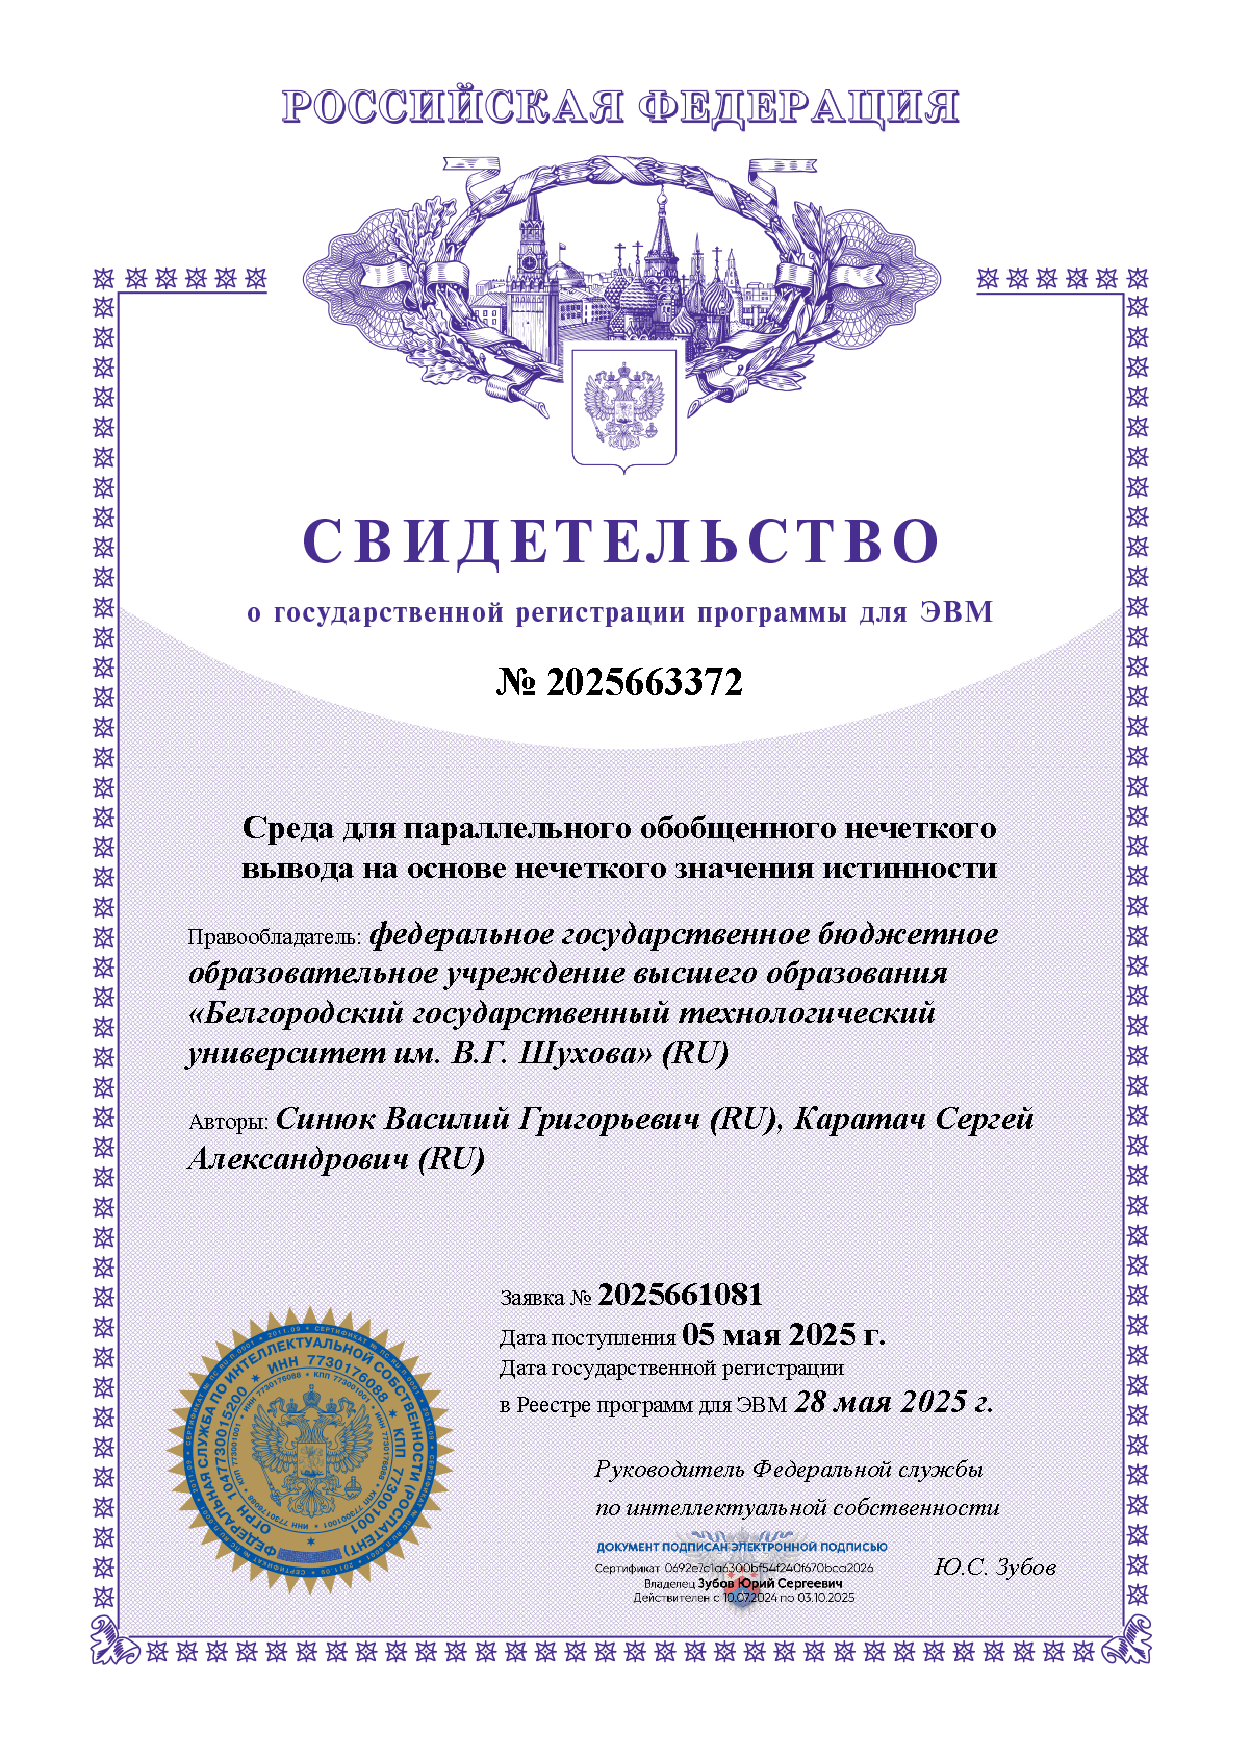
\includegraphics[width=0.9\textwidth, page=1]{images/RosPatent1.pdf}

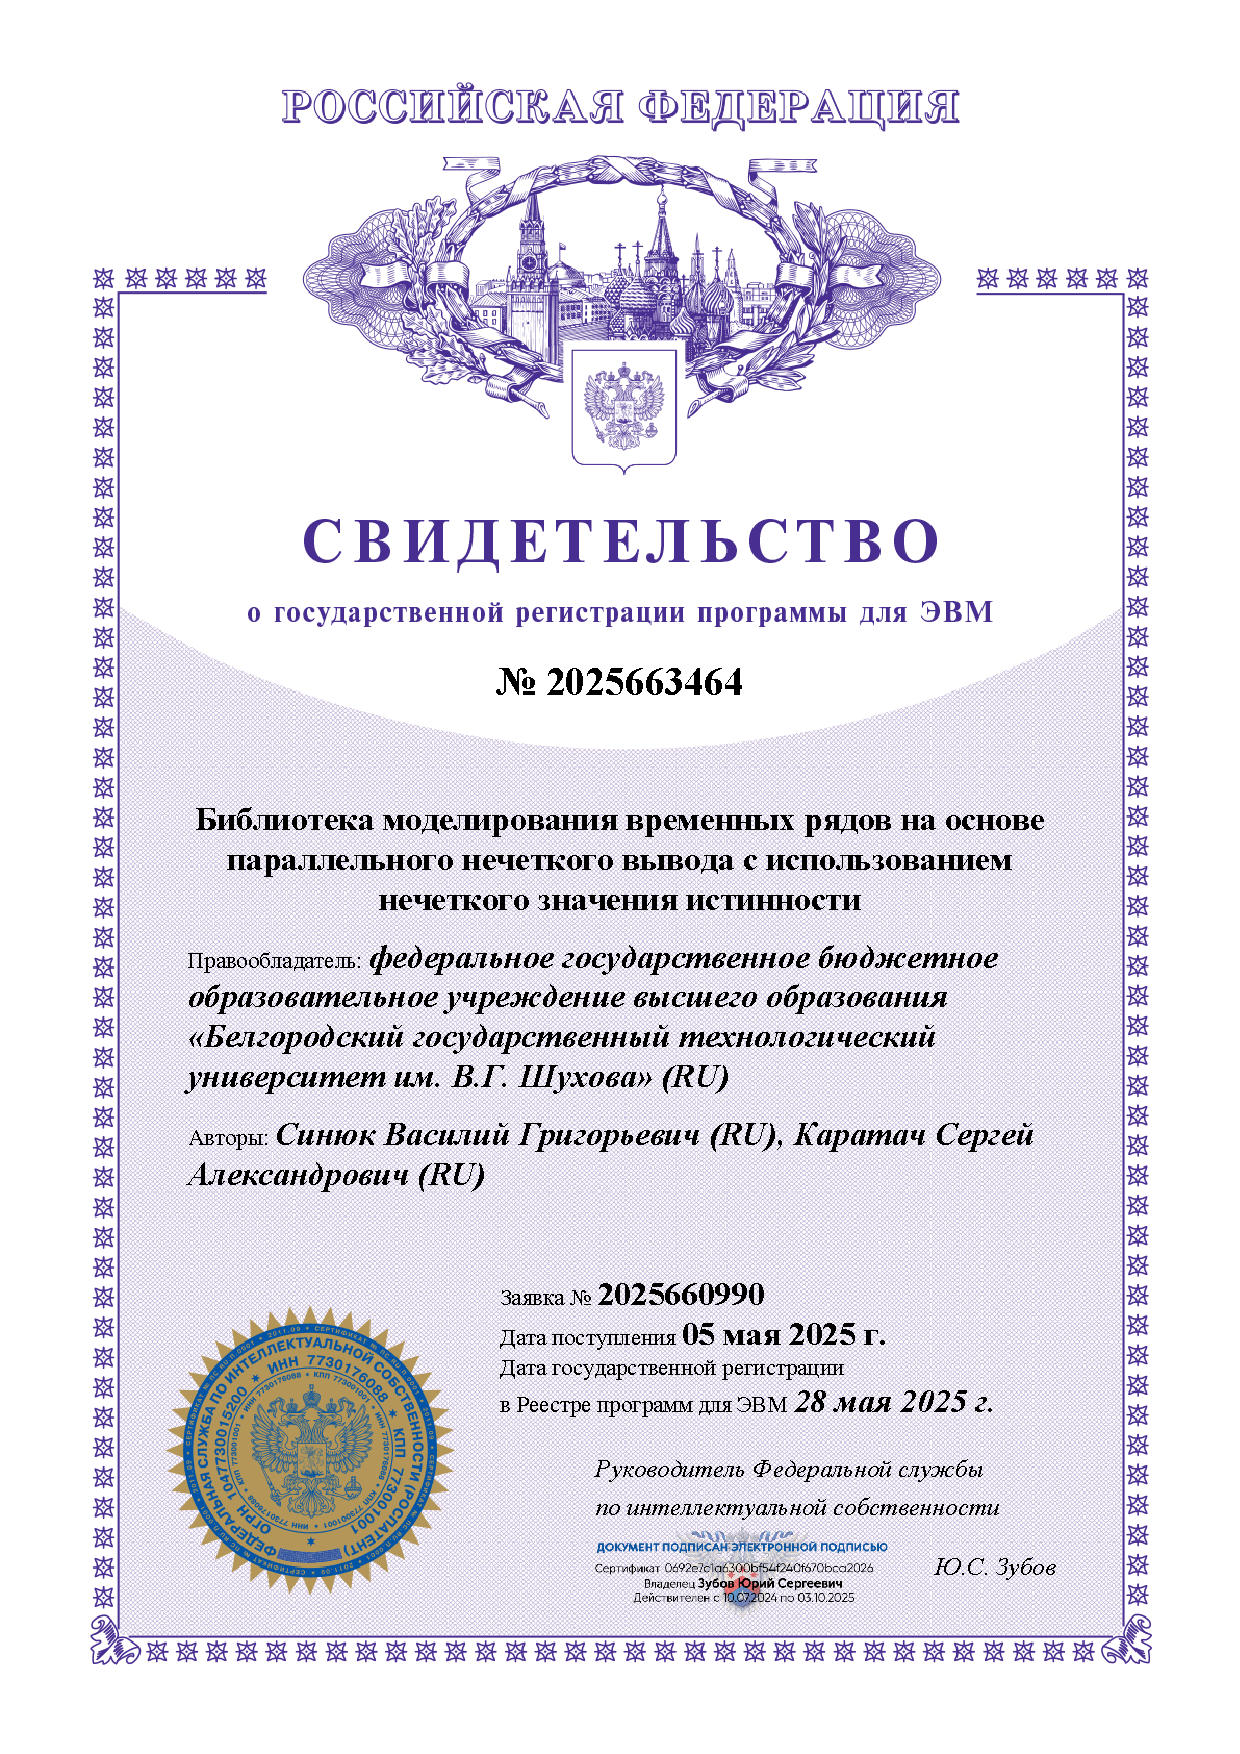
\includegraphics[width=0.9\textwidth, page=1]{images/RosPatent2.pdf}

%\chapter{Акт о внедрении результатов диссертационной работы в рабочий процесс}\label{app:C}

%\includepdf[pages=-]{images/act.pdf}
